\thepage
\section{Introduction}
In recent years open source software solutions have become widely popular and frequently used in both scientific and enterprise use, which can be attributed to a number of factors, most importantly the ease of development and deployment of IT projects, improved cybersecurity and enhanced scalability \cite{pwcLeadingBenefitsOpensource2016}. This increases the contribution to open source projects from enterprises and individuals alike. Due to its nature, open source software projects are driven by community contributions, and depend heavily on active participation in all phases of the project. Because there is a high dependency on the community in open source software projects, by understanding how contributions are included and what patterns emerge we can gain valuable insight into the project's current state and its trajectory.

\dots

% Summary of background literature and state of the art solutions
\section{Related work}
Software development in a corporate environment usually follows a strict hierarchial structure, where each participant is given a precise position and responsibility, like project manager, scrum master, senior or junior developer, and employees do not tend to work outside of their assigned tasks and territories. The main purpose of maintaining software development structures is for the company to ensure that the outcome of the project is in accordance with the business objective, adheres to the pre-set quality criteria and it is completed in a given timeframe; in other words to asses the risks associated with the business objective of the software project \cite{surekaUsingSocialNetwork2011}. This is achieved by breaking down the developed software into smaller, less complex components, and grouping the developers into managable teams, where the communication is moderated between teams \cite{birdLatentSocialStructure2008}. \\

% Open-source software development properties
On the other hand, Free/Libre Open Source Software (FLOSS) projects usually do not follow an organizational hierarchy, and are usually self-organizing and dynamic \cite{birdLatentSocialStructure2008}. Issues, bugs and progress are tracked openly, and everyone is encouraged to contribute based on the current topics and expertise, but purely on a volunteering basis. The lack of access restriction to certain modules allows for much more spontaneous interaction between developers, which generate large, complex networks \cite{martinez-romoUsingSocialNetwork2008}. These complex networks can be seen as large social networks of developers based on collaboration.

The collaboration networks of open source software (OSS) have been a subject of many academic research. Raymond \cite{crowstonSocialStructureFree2005} has defined collaboration based on bug report interaction, and observed the collaboration network of 124 large-scale SourceForge projects. The generated networks have widely different centralization properties, but it was observed that larger sized projects tend to be more decentralized. The broad community roles contributors tend to take have been also identified in \cite{crowstonSocialStructureFree2005}, which have been coined as the \textit{onion model} in \cite{martinez-romoUsingSocialNetwork2008} (Figure \ref{fig:onion1}).

\begin{figure}
    \centering
    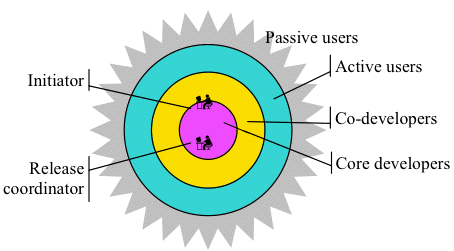
\includegraphics[width=0.6\textwidth]{figures/onion_model.png}
    \caption{The onion model of collaboration types in FLOSS projects \cite{crowstonSocialStructureFree2005}.}
    \label{fig:onion1}
\end{figure}
%\citeauthor{raymondCathedralBazaar1998} 

% Onion model
% No definitive
\begin{itemize}
    \item Open-source software development properties
    \begin{itemize}
        \item centralized vs decentralized
        \item No collocation
        \item Enterprise support
        \item Version control, issue tracking
    \end{itemize}
    \item Relevant social aspects of OS projects
    \item State of the art
    \begin{itemize}
        \item Collaboration by coediting files
        \item Contributors form dynamic social networks
        \item Problem of analysing changes over time in a network
        \item Other studies in this field...
    \end{itemize}
    \item Preliminary analysis results (pandas, networkx, \dots)
\end{itemize}


\section{Motivation of research problem and research question}

\begin{itemize}
    \item Importance of OS project analysis based on lit rew
    \item Analysing effects of large events within the lifecycle of the OS project in order to improve them or adapt
    \begin{itemize}
        \item Planned, foreseeable changes (e.g. upcoming major release)
        \item Unforeseeable changes (e.g. end of support, pandemic)
    \end{itemize}
    \item Research questions
    \begin{itemize}
        \item What social patterns emerge within large-scale open-source software projects?
        \begin{itemize}
            \item Are there smaller "core" collaborator networks connected with weak links or do they form one large interconnected network?
            \item Are there usually key contributors, who are central to the project and collaborate with most contributors, or is it completely decentralized?
            \item How does the size of the project change these properties?
        \end{itemize}
        \item How does the structure of OS software development collaboration change over time?
        \begin{itemize}
            \item Are there any major changes over the natural project lifecycle? Are they visible in the collaboration network? (e.g. planning, developing, bugfixing, sunset?)
            \item How does a sudden major event change the participation and development?
        \end{itemize}
    \end{itemize}
\end{itemize}


\section{Proposed research method}

\begin{itemize}
    \item Developing a tool, that can extract the collaboration information from any OS project (from GitHub/git repository)
    \item Data cleaning - method to merge authors, excluding common folders, etc\dots
    \item Qualitative research
    \begin{itemize}
        \item Observing collaboration statistics and networks in order to discover patterns: connected components, centrality, changes over time
    \end{itemize}
    \item Quantitative research
    \begin{itemize}
        \item Composing a large set of repositories (different sizes, properties)
        \item Detecting past changes automatically based on changes in measured statistics
    \end{itemize}
\end{itemize}

\section{Outline of thesis}
\begin{itemize}
    \item Literature review
    \begin{itemize}
        \item Network analysis, relevant metrics
        \item Properties of social collaboration networks
    \end{itemize}
    \item Used repositories, selection criteria
    \item Data cleaning - files, authors, max modifications
    \item Implementation
    \begin{itemize}
        \item \dots
    \end{itemize}
    \item Qualitative analysis
    \item Quantitative analysis
    \item Conclusion
\end{itemize}

\subsection{(Preliminary literature list - in references)}

\subsection{Work plan including milestones}

\begin{itemize}
    \item Data cleaning - files, authors, max modifications
    \item Implementation
    \begin{itemize}
        \item \dots
    \end{itemize}
    \item Qualitative analysis
    \item Quantitative analysis
    \item Conclusion
\end{itemize}